\documentclass{article}

\usepackage{geometry}
\usepackage[russian]{babel}
\usepackage[utf8]{inputenc}
\usepackage{graphicx}
\usepackage{amsmath}
\usepackage{pgfplotstable}

\newgeometry{scale = 0.8}
\selectlanguage{russian}
\setcounter{tocdepth}{5}
\renewcommand{\thesection}{\Roman{section}} 

\title{Лабораторная работа 4.3.2\\ Дифракция света на ультразвуковой волне в жидкости\\ Отчёт о выполнении}
\date{2018-02-10}
\author{Дерека С.А., группа 642}


\begin{document}

\maketitle
\pagenumbering{gobble}
\newpage
\pagenumbering{arabic}

\section{Цель, оборудование}
\begin{itemize}
	\item \textbf{Цель работы:} изучение дифракции света на синусоидальной акустической решётке и наблюдение фазовой решётки методом тёмного поля.
	\item \textbf{В работе используется:} оптическая скамья, осветитель, два длиннофокусных объектива, кювета с жидкостью, кварцевый излучатель с микрометрическим винтом, генератор ультразвуковой частоты, линза, вертикальная нить на рейтере, микроскоп.
\end{itemize}


\section{Схема установки}
\begin{figure}[h!]
  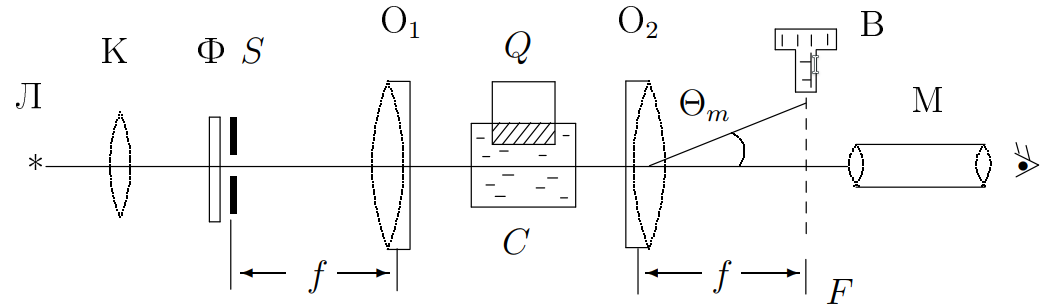
\includegraphics[width=\linewidth]{pic1.png}
  \caption{Схема установки для наблюдения дифракции на акустической решётке}
  \label{fig:pic1}
\end{figure}
\begin{figure}[h!]
  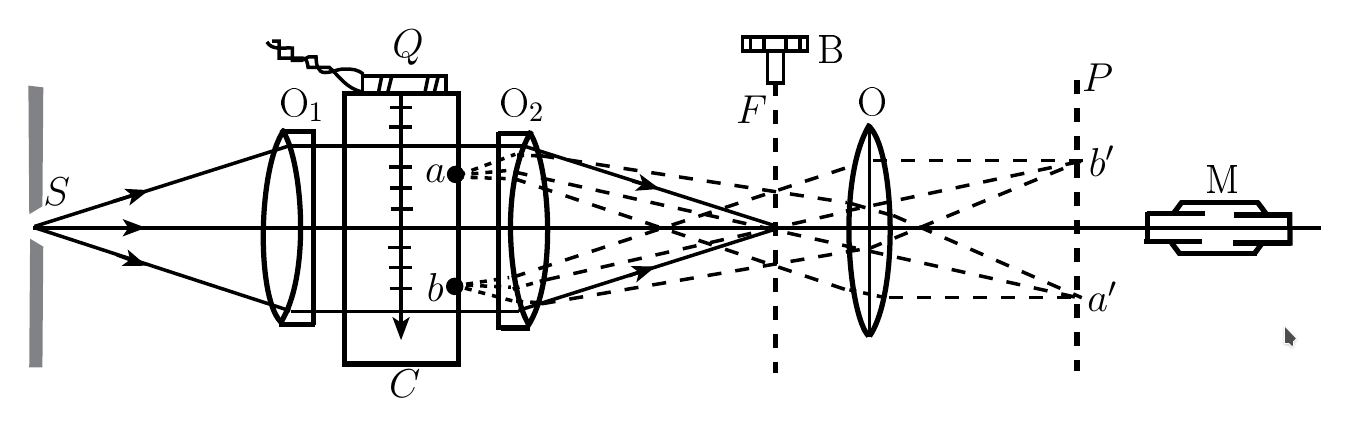
\includegraphics[width=\linewidth]{pic2.png}
  \caption{Схема установки для наблюдения акустической решётки методом тёмного поля}
  \label{fig:pic2}
\end{figure}
\textbf{Обозначения для рис. \ref{fig:pic1} и \ref{fig:pic2}}
\begin{itemize}
	\item Q - ультразвуковой излучатель
	\item $O_2$ - камерный объектив
	\item M - микроскоп
	\item B  - микрометрический винт
	\item S  - щель
\end{itemize}
\textbf{Параметры установки:}
\begin{itemize}
	\item f = 28 см
	\item $\lambda$ = 6400 $\pm$ 200 {\AA}
\end{itemize}


\section{Теоретические сведения}
Длина $\Lambda$ ультразвуковой волны определяется соотношением:
\begin{equation}
	\Lambda\sin{\Theta_m} = m\lambda
\end{equation}
В силу малости углов $\Theta_m$ окончательное соотношение может быть представлено в виде:
\begin{equation}
	l_m = mf\frac{\lambda}{\Lambda}
\end{equation}
где $l_m$ - измеренное на опыте расстояние между m-ым и нулевым максимумами, а f - фокусное расстояние $O_2$.
Скорость $v$ распространения звука в воде можно рассчитать, если известна частота кварцевого излучателя $\nu$:
\begin{equation}
	v = \lambda\nu
\end{equation}


\section{Определение скорости ультразвука по дифракционной картине}
\begin{table}[h!]
\centering
\caption{}
\label{table1}
\begin{tabular}{|l|l|l|l|l|}
\hline
   & \multicolumn{4}{l|}{$\nu$, МГц} \\ \hline
   & 1.005  & 1.132  & 1.256 & 1.841 \\ \hline
m  & \multicolumn{4}{l|}{Y, дел}     \\ \hline
-2 & 18     & 16     & 10    &       \\ \hline
-1 & 52     & 50     & 51    & 32    \\ \hline
0  & 88     & 87     & 90    & 89    \\ \hline
1  & 117     & 121     & 126    & 143    \\ \hline
2  & 150     & 158     & 161    &       \\ \hline
\end{tabular}
\end{table}
В таблице \ref{table1} приведены результаты измерений положений максимумов в зависимости от частоты излучателя. $\sigma_{\nu}$ = 0.005 Мгц, $\sigma_Y$ = 2 дел.
\begin{figure}[h!]
  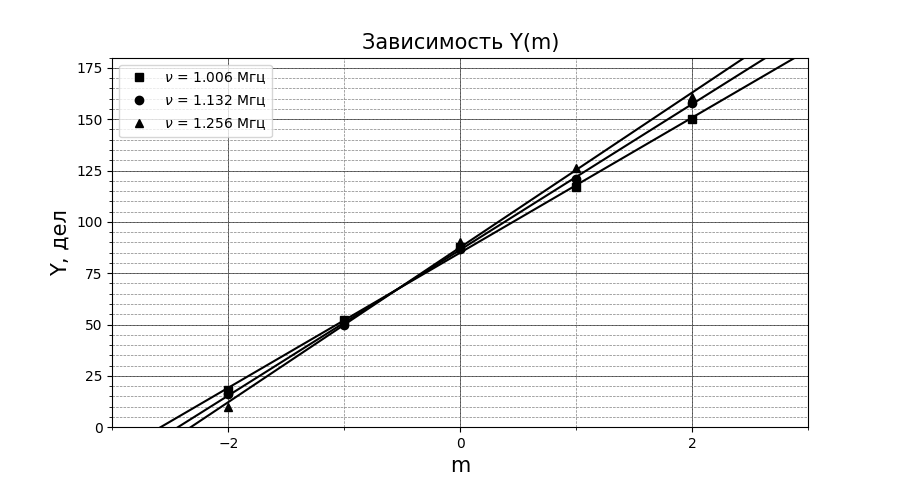
\includegraphics[width=\linewidth]{Figure_1.png}
  \caption{График зависимости Y(m)}
  \label{fig:graph1}
\end{figure}
На рисунке \ref{fig:graph1} представлен график зависимости положения максимума Y от его номера m при разных частотах $\nu$.
\begin{table}[]
\centering
\caption{}
\label{table2}
\begin{tabular}{|l|l|l|l|l|l|}
\hline
$\nu$, МГц & k, дел & $\sigma_k$, дел & $\Lambda,10^{-3}$ м & $v, 10^3$ м/с & $\sigma_v, 10^3$ м/с \\ \hline
1.006      & 32.9   & 0.2             & 1.33               & 1.51                 & 0.06                        \\ \hline
1.132      & 35.5   & 0.3             & 1.29               & 1.48                 & 0.07                        \\ \hline
1.256      & 37.7   & 0.2             & 1.18               & 1.45                 & 0.07                        \\ \hline
\end{tabular}
\end{table}
В таблице \ref{table2} представлен результат расчёта длины волны $\Lambda$ и скорости звука $v$ по угловым коэффициентам k.
Вычислим среднюю скорость распространения звука: $<v>$ = 1.48 м/c;
$\sigma_v=\sqrt{\sigma_{vr}^2+\sigma_{vm}^2}$ = 0.07 м/с


\section{Определение скорости ультразвука методом тёмного поля}
\begin{table}[h!]
\centering
\caption{}
\label{table3}
\begin{tabular}{|l|l|l|l|l|l|l|}
\hline
$\nu$, МГц & a, дел & b, дел & с, дел & $l_m$, дел & $1/\nu$, с & L, $10^{-3}$ м \\ \hline
1.01       & 0      & 2      & 7      & 0.286      & 0.990      & 1.465          \\ \hline
1.788      & 2      & 3.1    & 7      & 0.157      & 0.559      & 0.878          \\ \hline
1.42       & 3      & 5      & 5      & 0.400      & 0.704      & 1.042          \\ \hline
1.525      & 3.1    & 5      & 5      & 0.380      & 0.656      & 0.970          \\ \hline
\end{tabular}
\end{table}
В таблице \ref{table3} приведены рассчитанные по параметрам решётки значения длин ультразвуковых волн.
\begin{figure}[h!]
  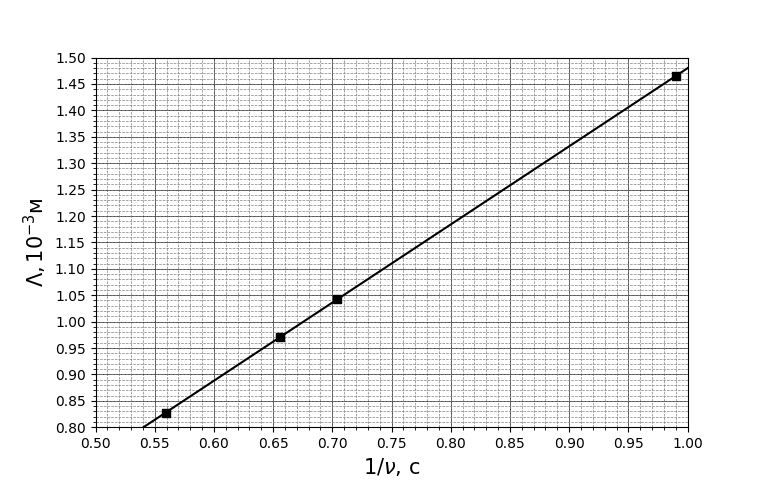
\includegraphics[width=\linewidth]{Figure_2.png}
  \caption{График зависимости длины волны $\Lambda$ от периода}
  \label{fig:graph2}
\end{figure}
По графику \ref{fig:graph2} рассчитываем угловой коэффициент прямой: k = (1.5 $\pm$ 0.2) $10^3$ м/c\\
Согласно формуле (3) это и есть искомая скорость.


\section{Результаты и выводы}
В ходе работы удалось наблюдать дифракцию света на акустической решётке (дифракционную картину и саму решётку методом тёмного поля). На основе данных, полученных в ходе измерений, была определена с достаточно высокой точностью скорость распространения звуковых волн в воде.
\begin{table}[h!]
\centering
\caption{}
\label{table4}
\begin{tabular}{|l|l|l|l|}
\hline
Метод                 & $v, 10^3$ м/с & $\sigma_v, 10^3$ м/с & $v_{tab}, 10^3$ м/с \\ \hline
Дифракционная картина & 1.48          & 0.07                 & 1.485               \\ \hline
Тёмное поле           & 1.5           & 0.2                  & 1.485               \\ \hline
\end{tabular}
\end{table}
Полученные результаты приведены в таблице \ref{table4}.

\end{document}\grid
